\section{Utilizing graph eigenvectors [25 points]}

\begin{figure}[H]
	\centering
	\begin{subfigure}{0.5\textwidth}
		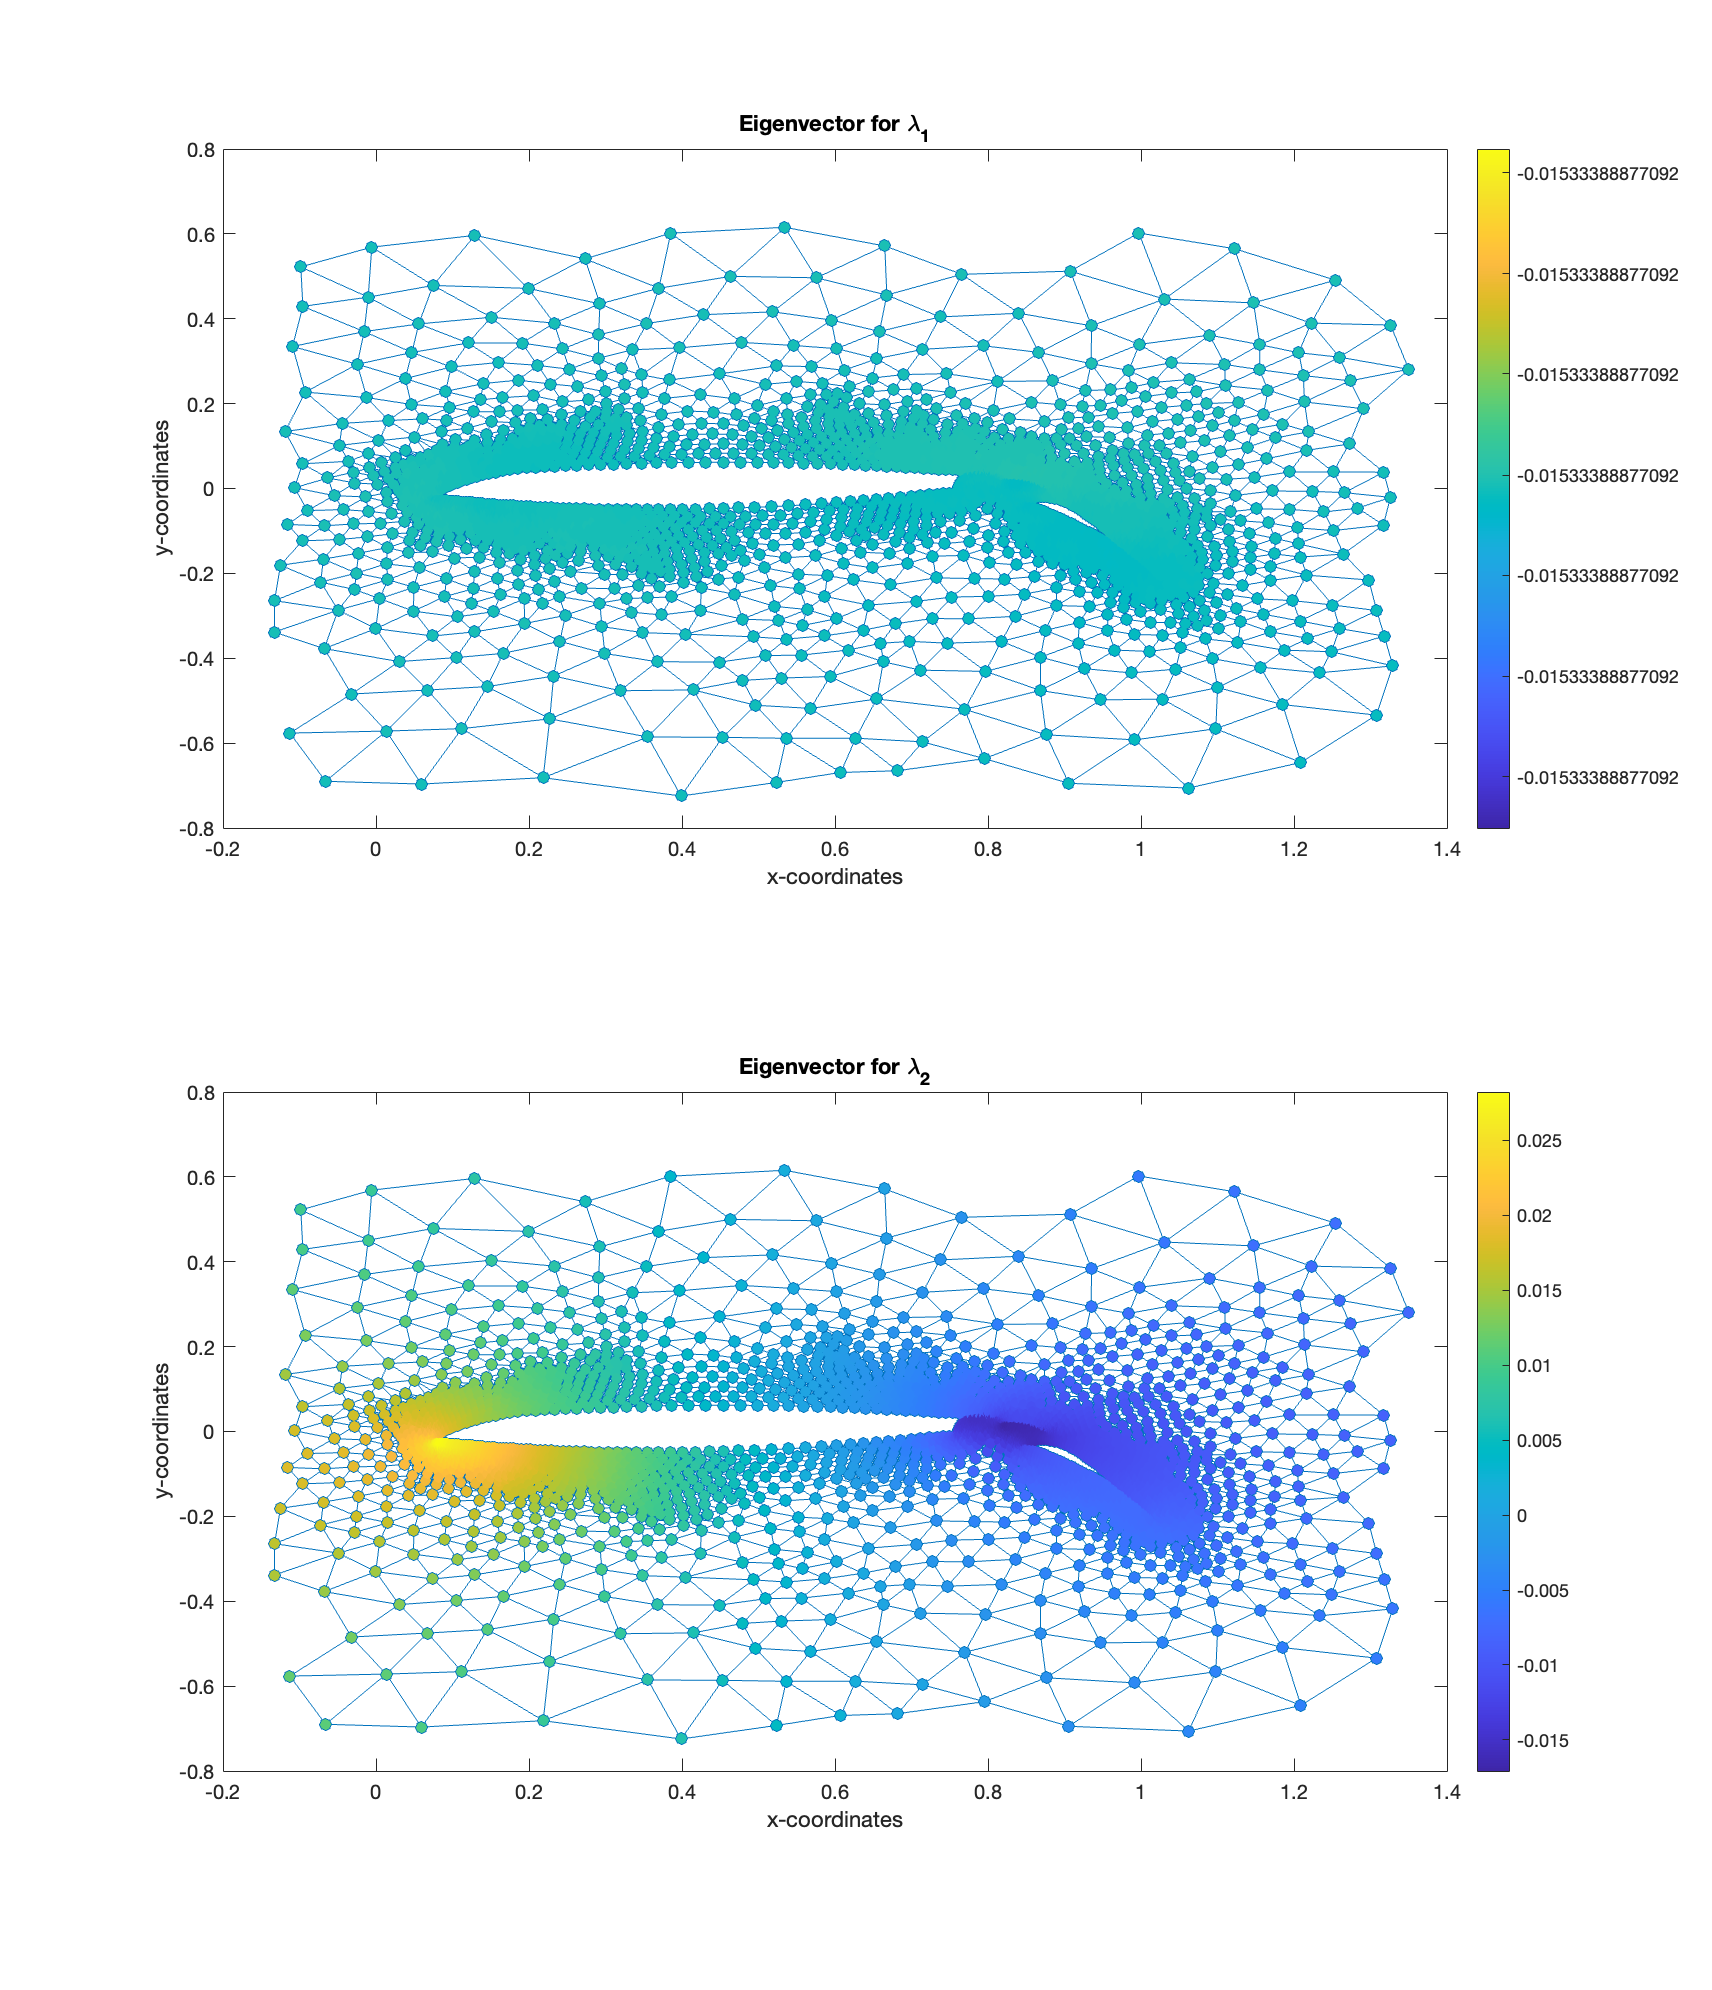
\includegraphics[width=\textwidth]{./media/eigenvector.png}
		\caption{mesh3e1}
		\label{fig:spec_crack}
	\end{subfigure}%
	~
	\begin{subfigure}{0.5\textwidth}
		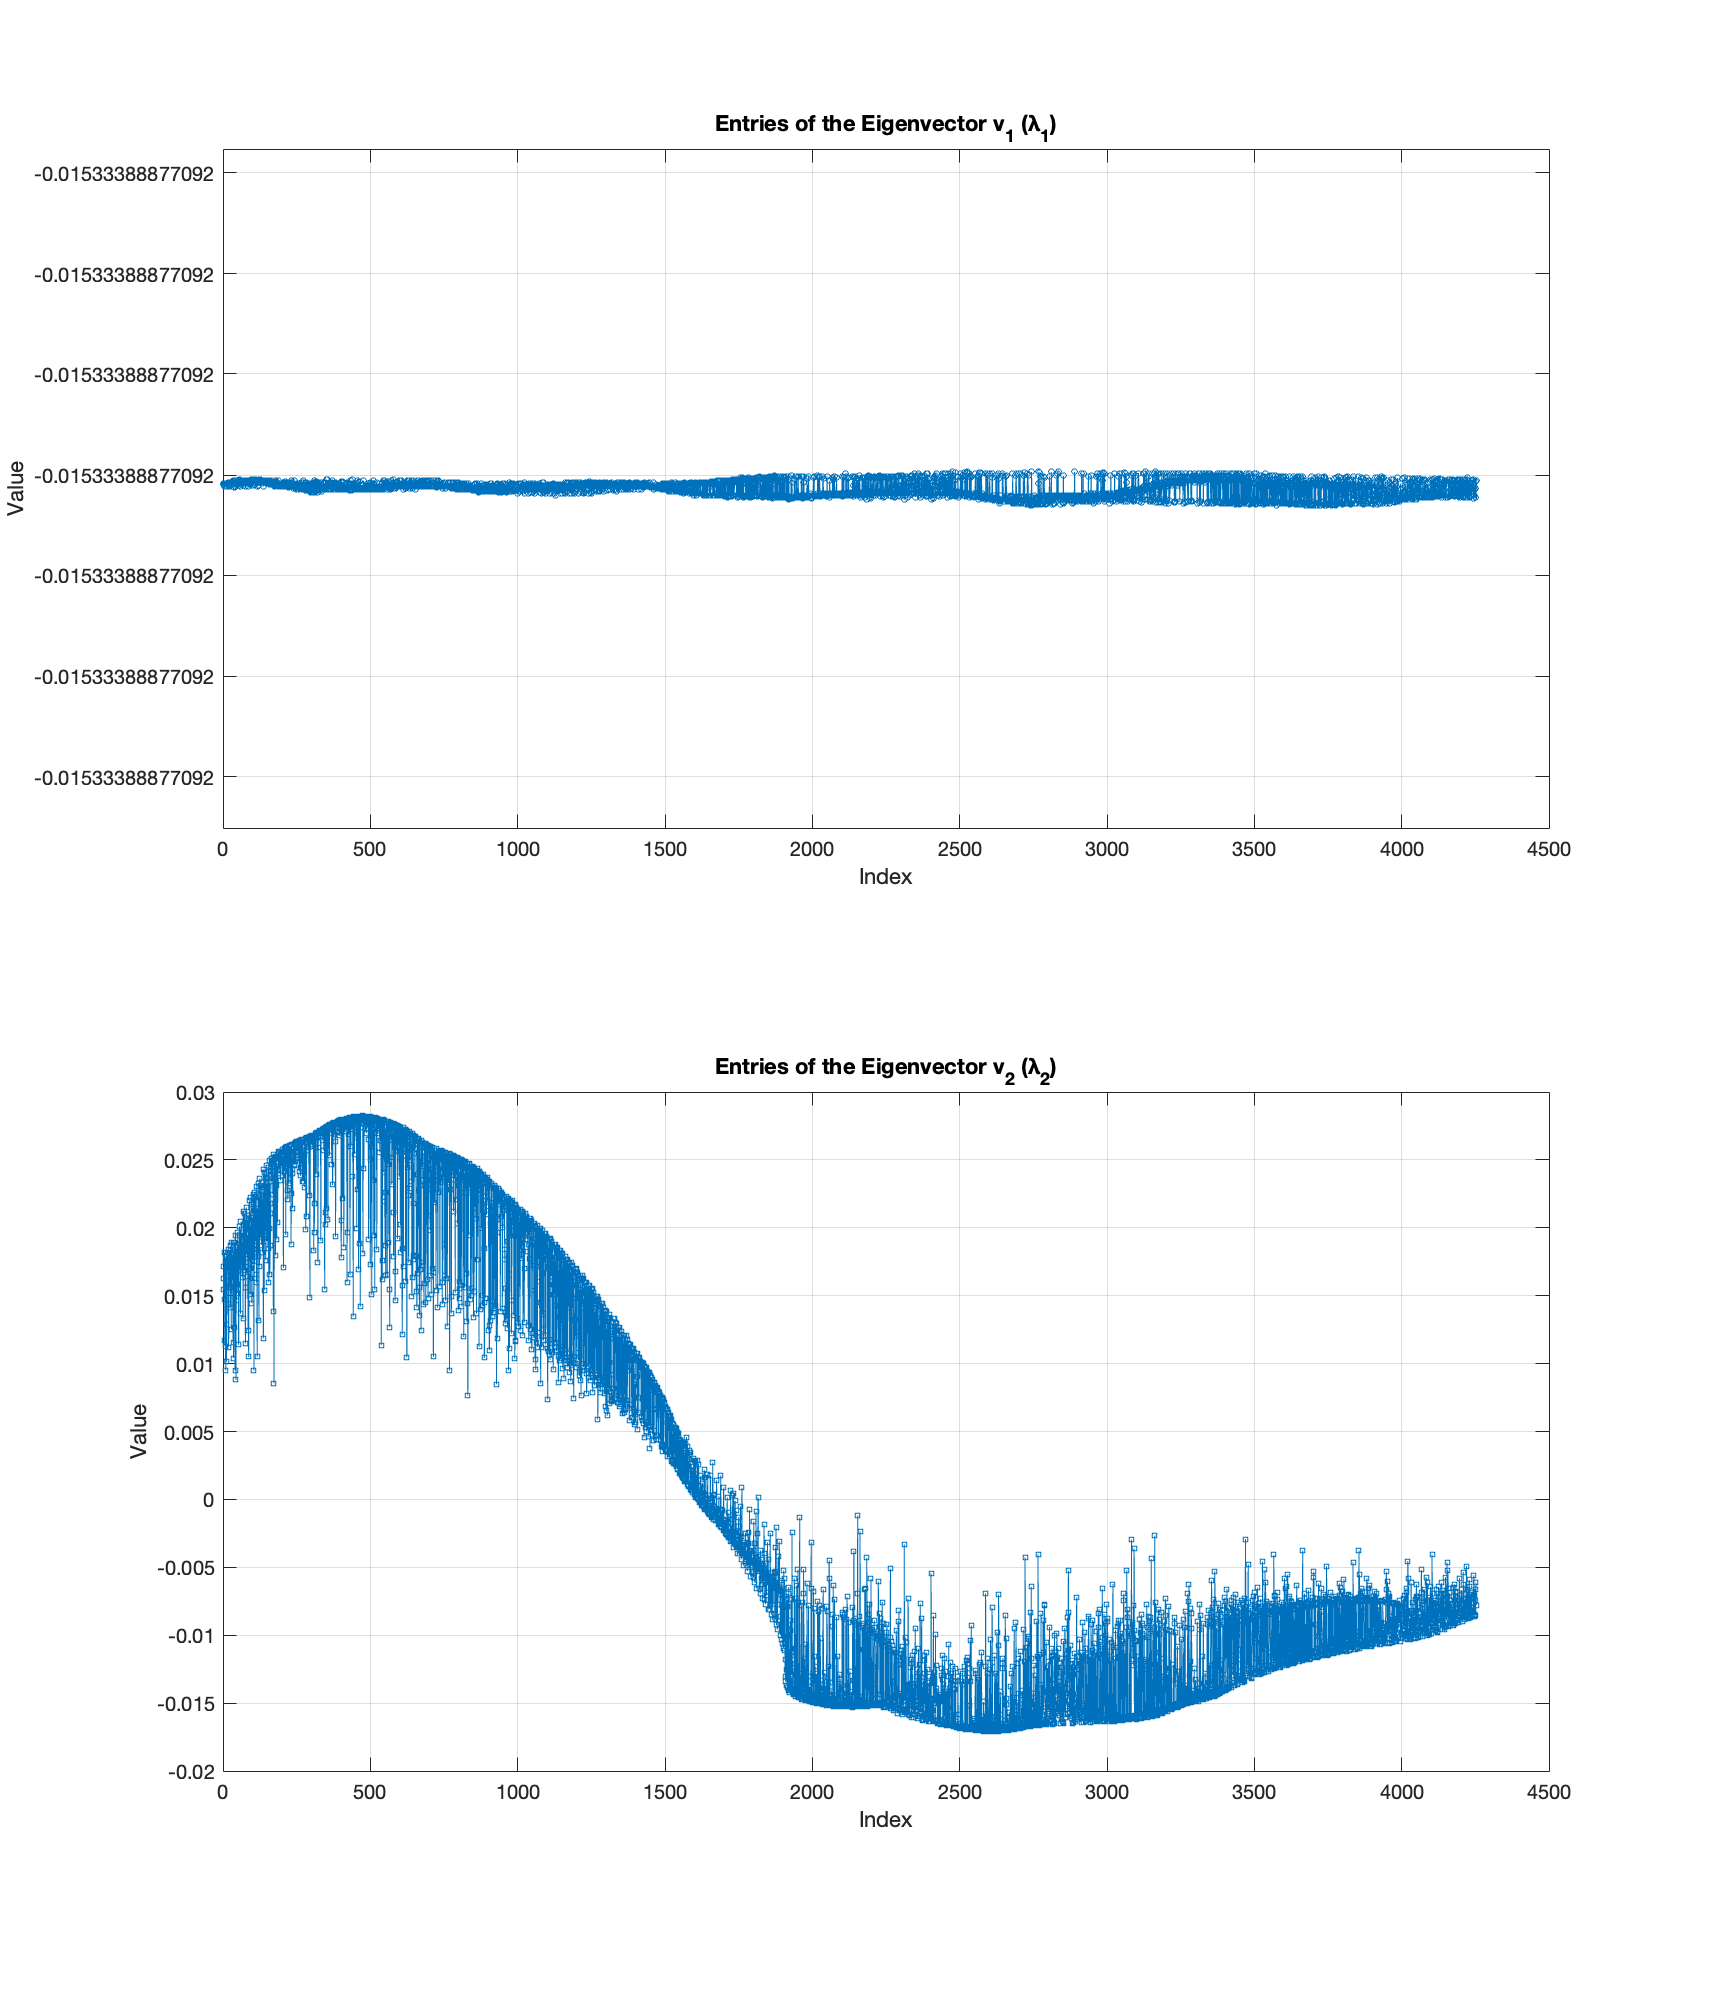
\includegraphics[width=\textwidth]{./media/eig_2.png}
		\caption{barth4}
		\label{fig:coord_crack}
	\end{subfigure}\\
	\caption{Spectral bi-partitioning results using the eigenvectors to supply coordinates (bottom) and using cartesian coordinates (top).}
	\label{fig:rec_bi}
\end{figure}

\begin{figure}[H]
	\centering
	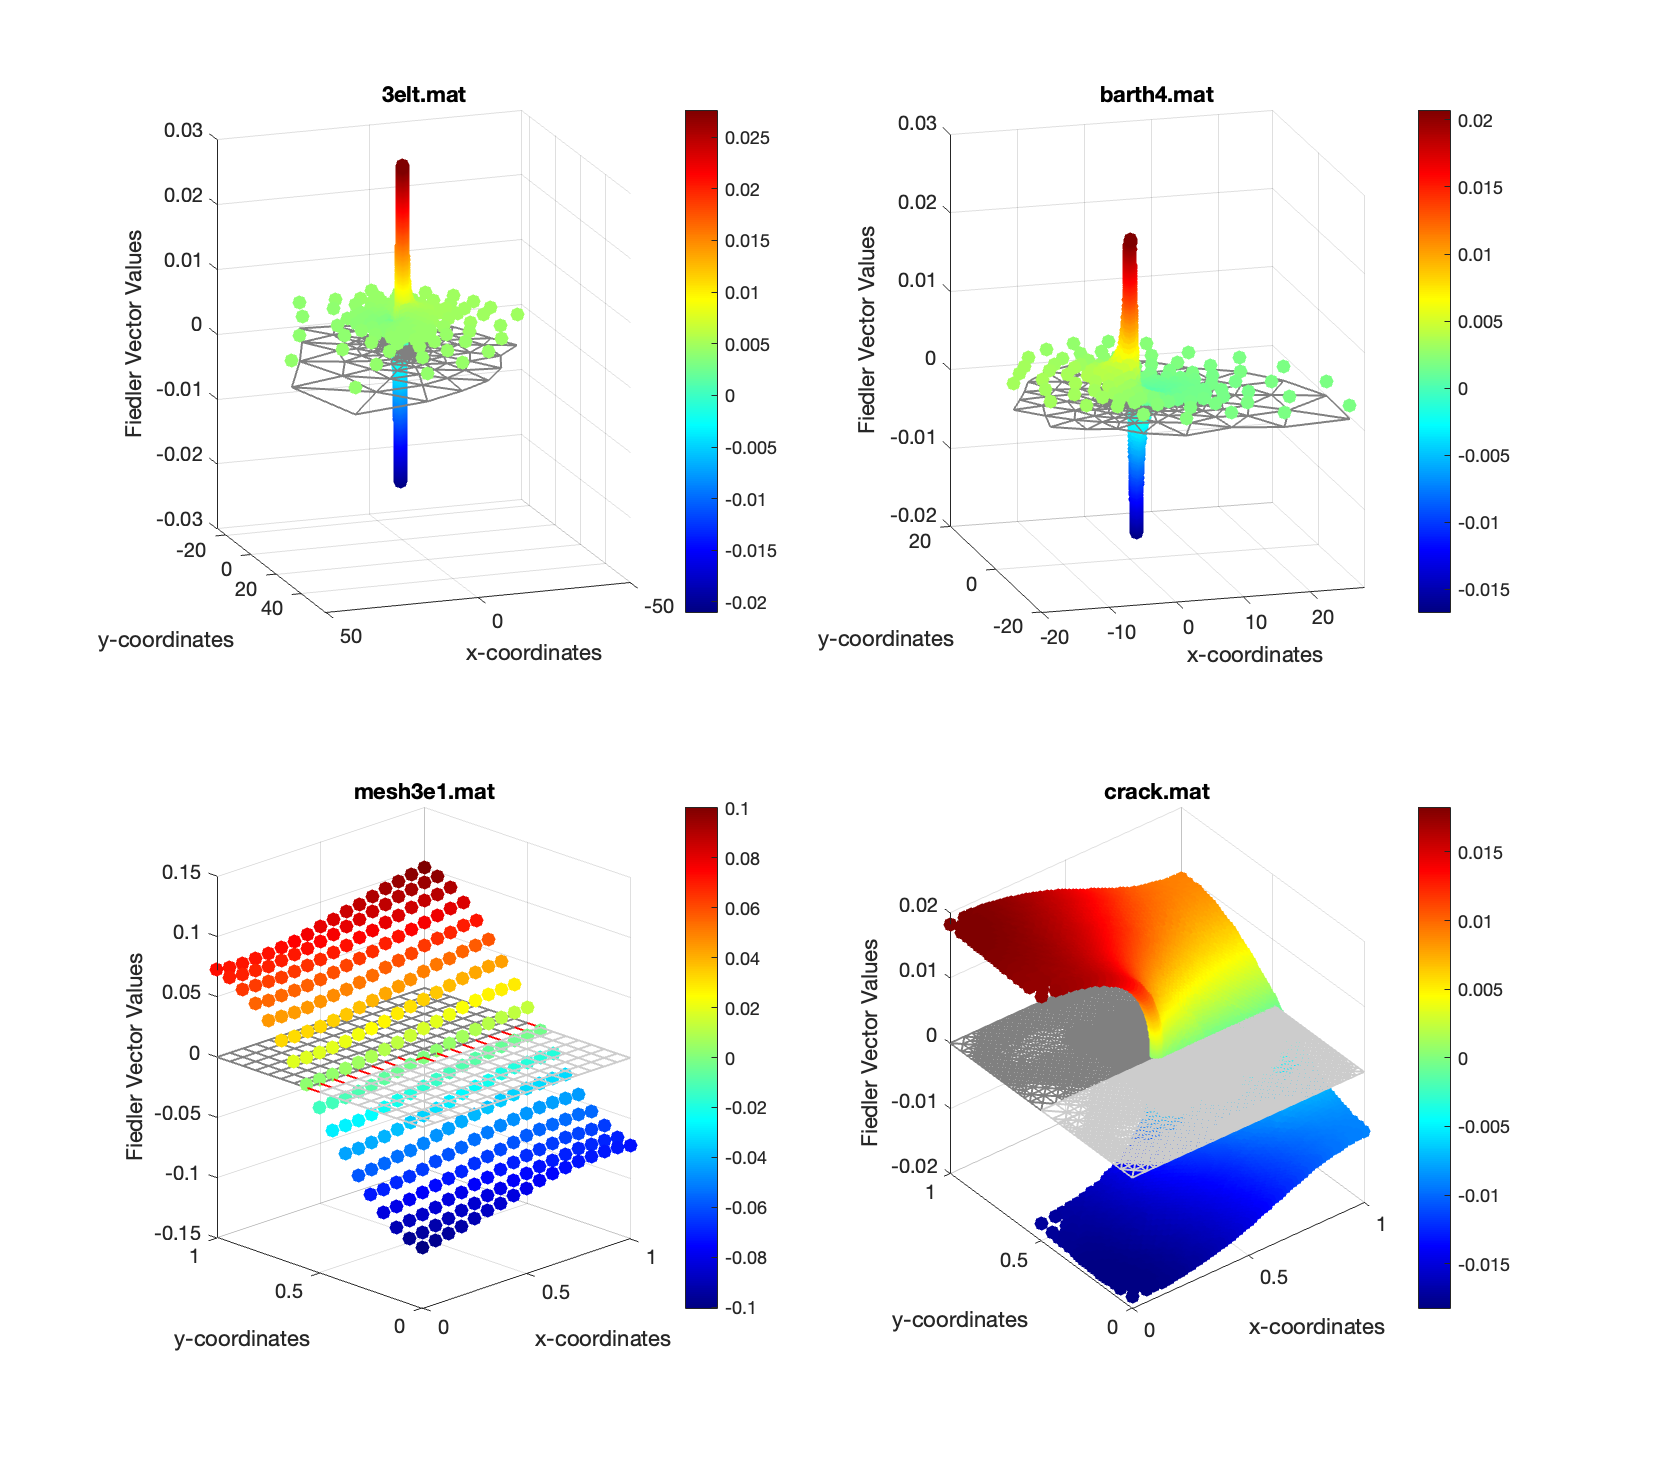
\includegraphics[width=\textwidth]{./media/fiedler.png}
	\caption{Entries of the eigenvector associated with the second smallest eigenvalue $\lambda_2$ of the Graph Laplacian matrix $L$}
	\label{fig:fied}
\end{figure}

\begin{figure}[H]
	\centering
	\begin{subfigure}{0.5\textwidth}
		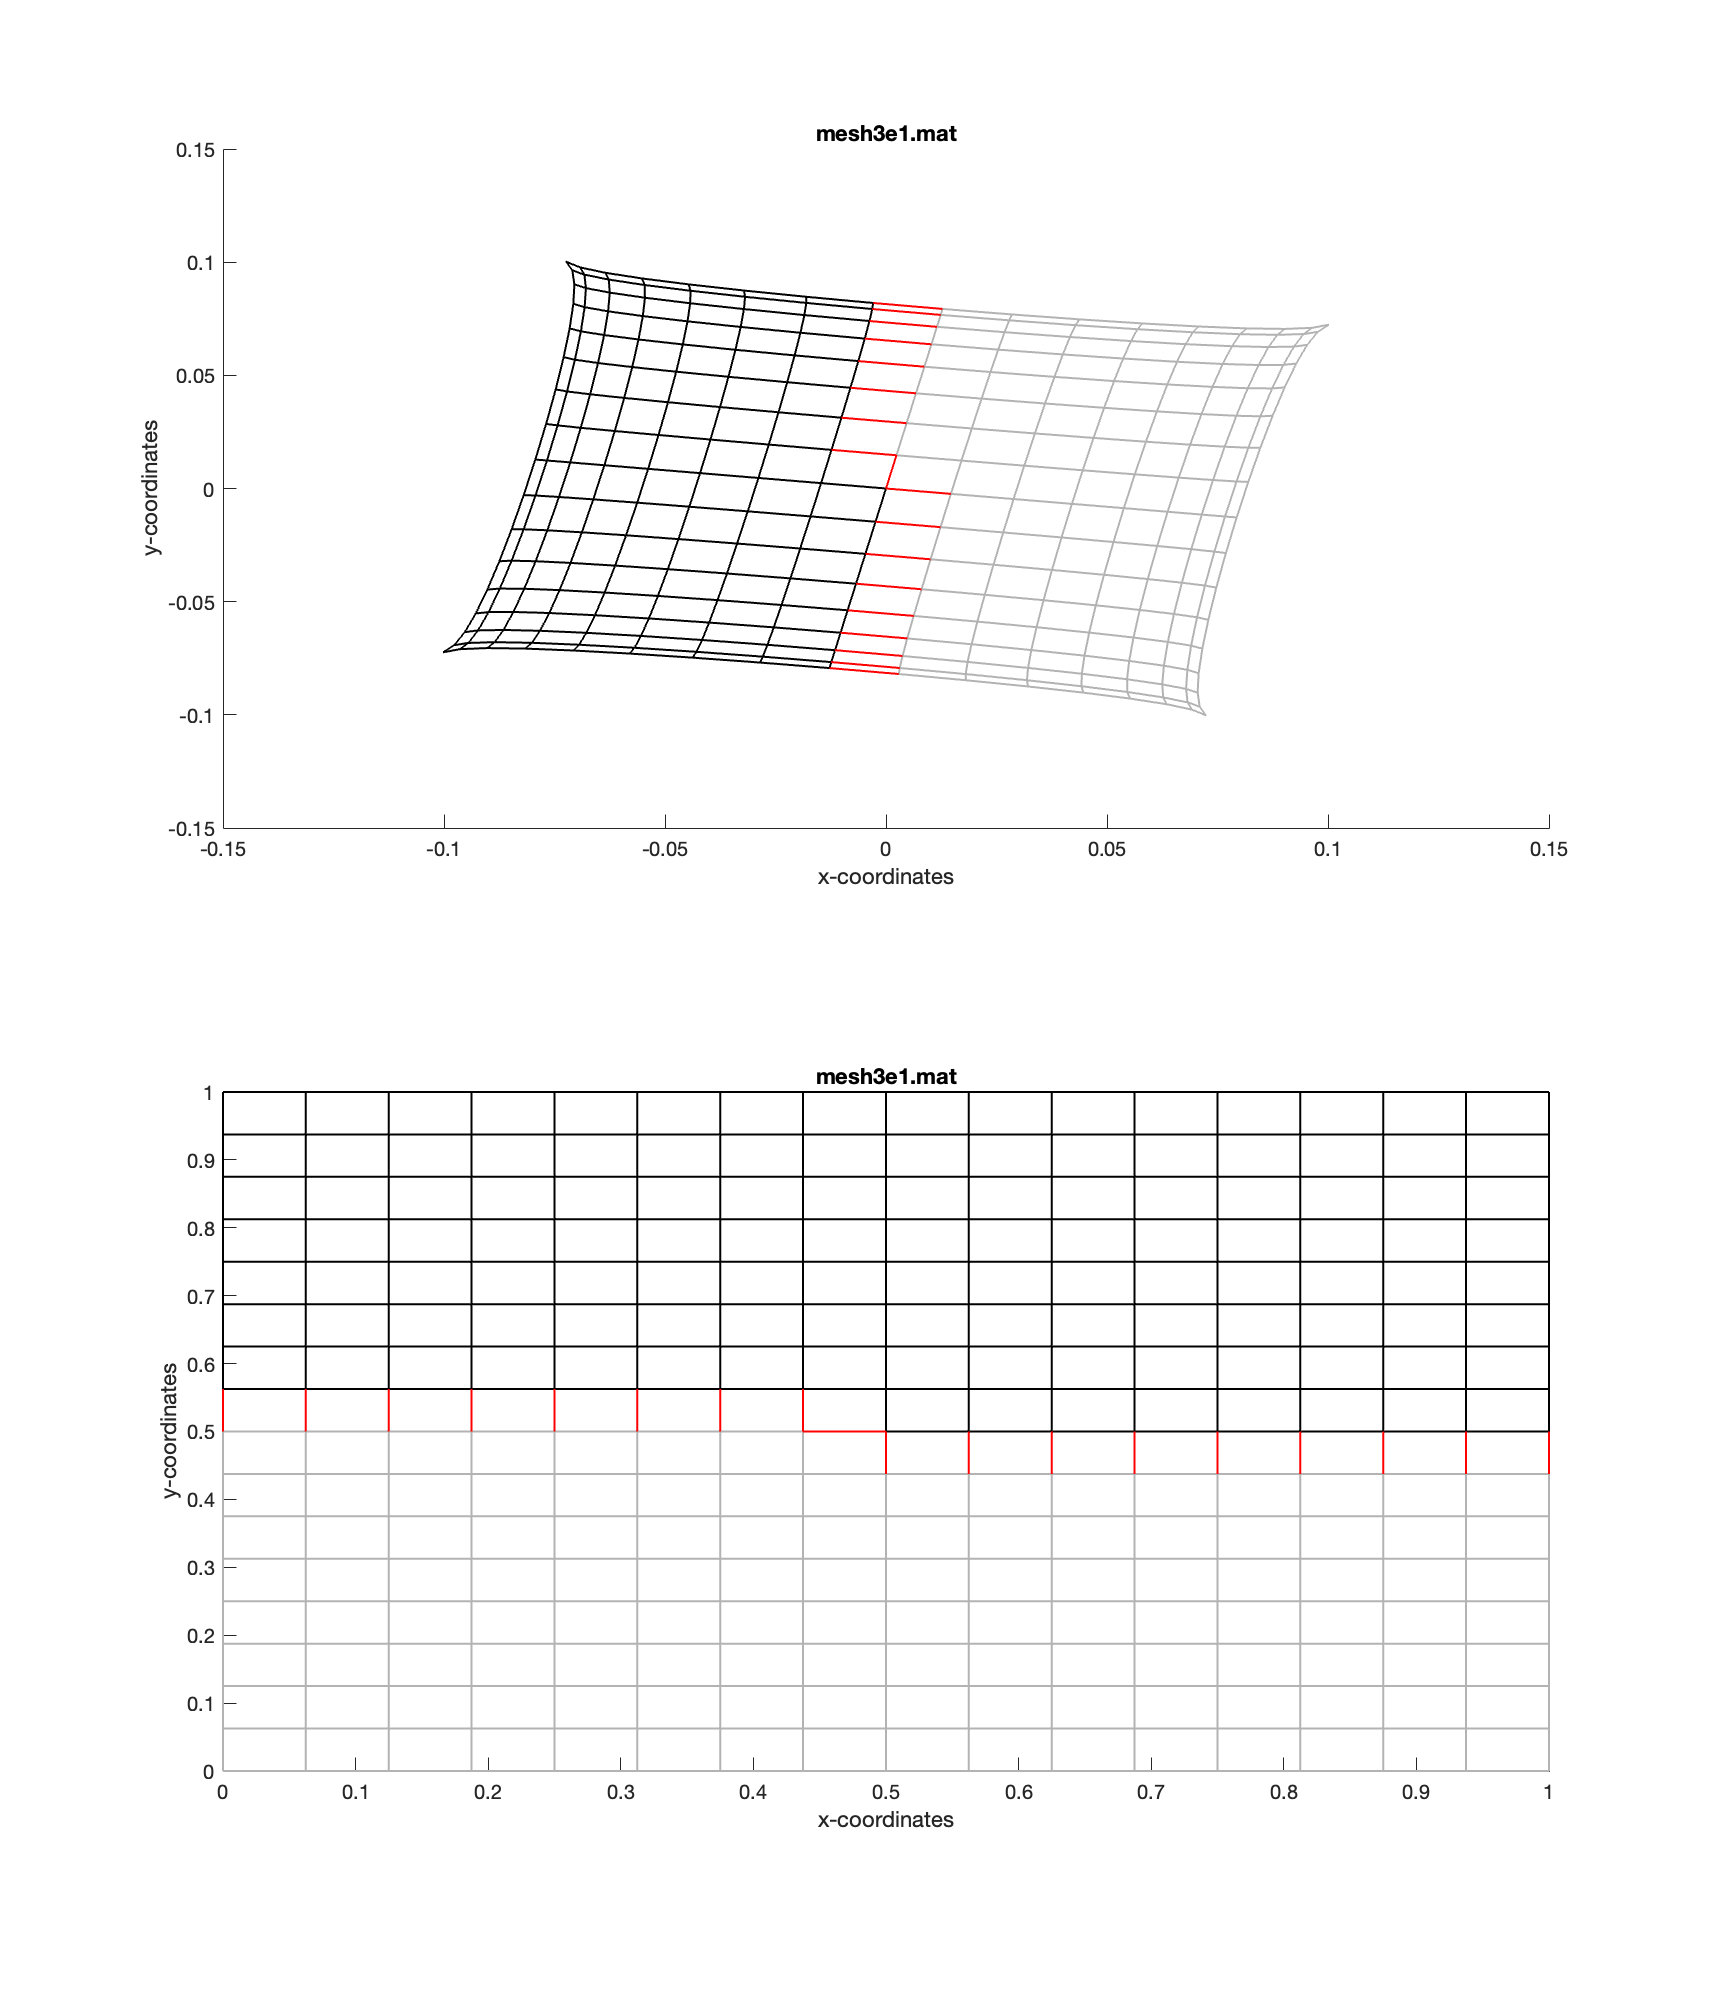
\includegraphics[width=\textwidth]{./media/mesh3e1_eigen.png}
		\caption{mesh3e1}
		\label{fig:spec_crack}
	\end{subfigure}%
	~
	\begin{subfigure}{0.5\textwidth}
		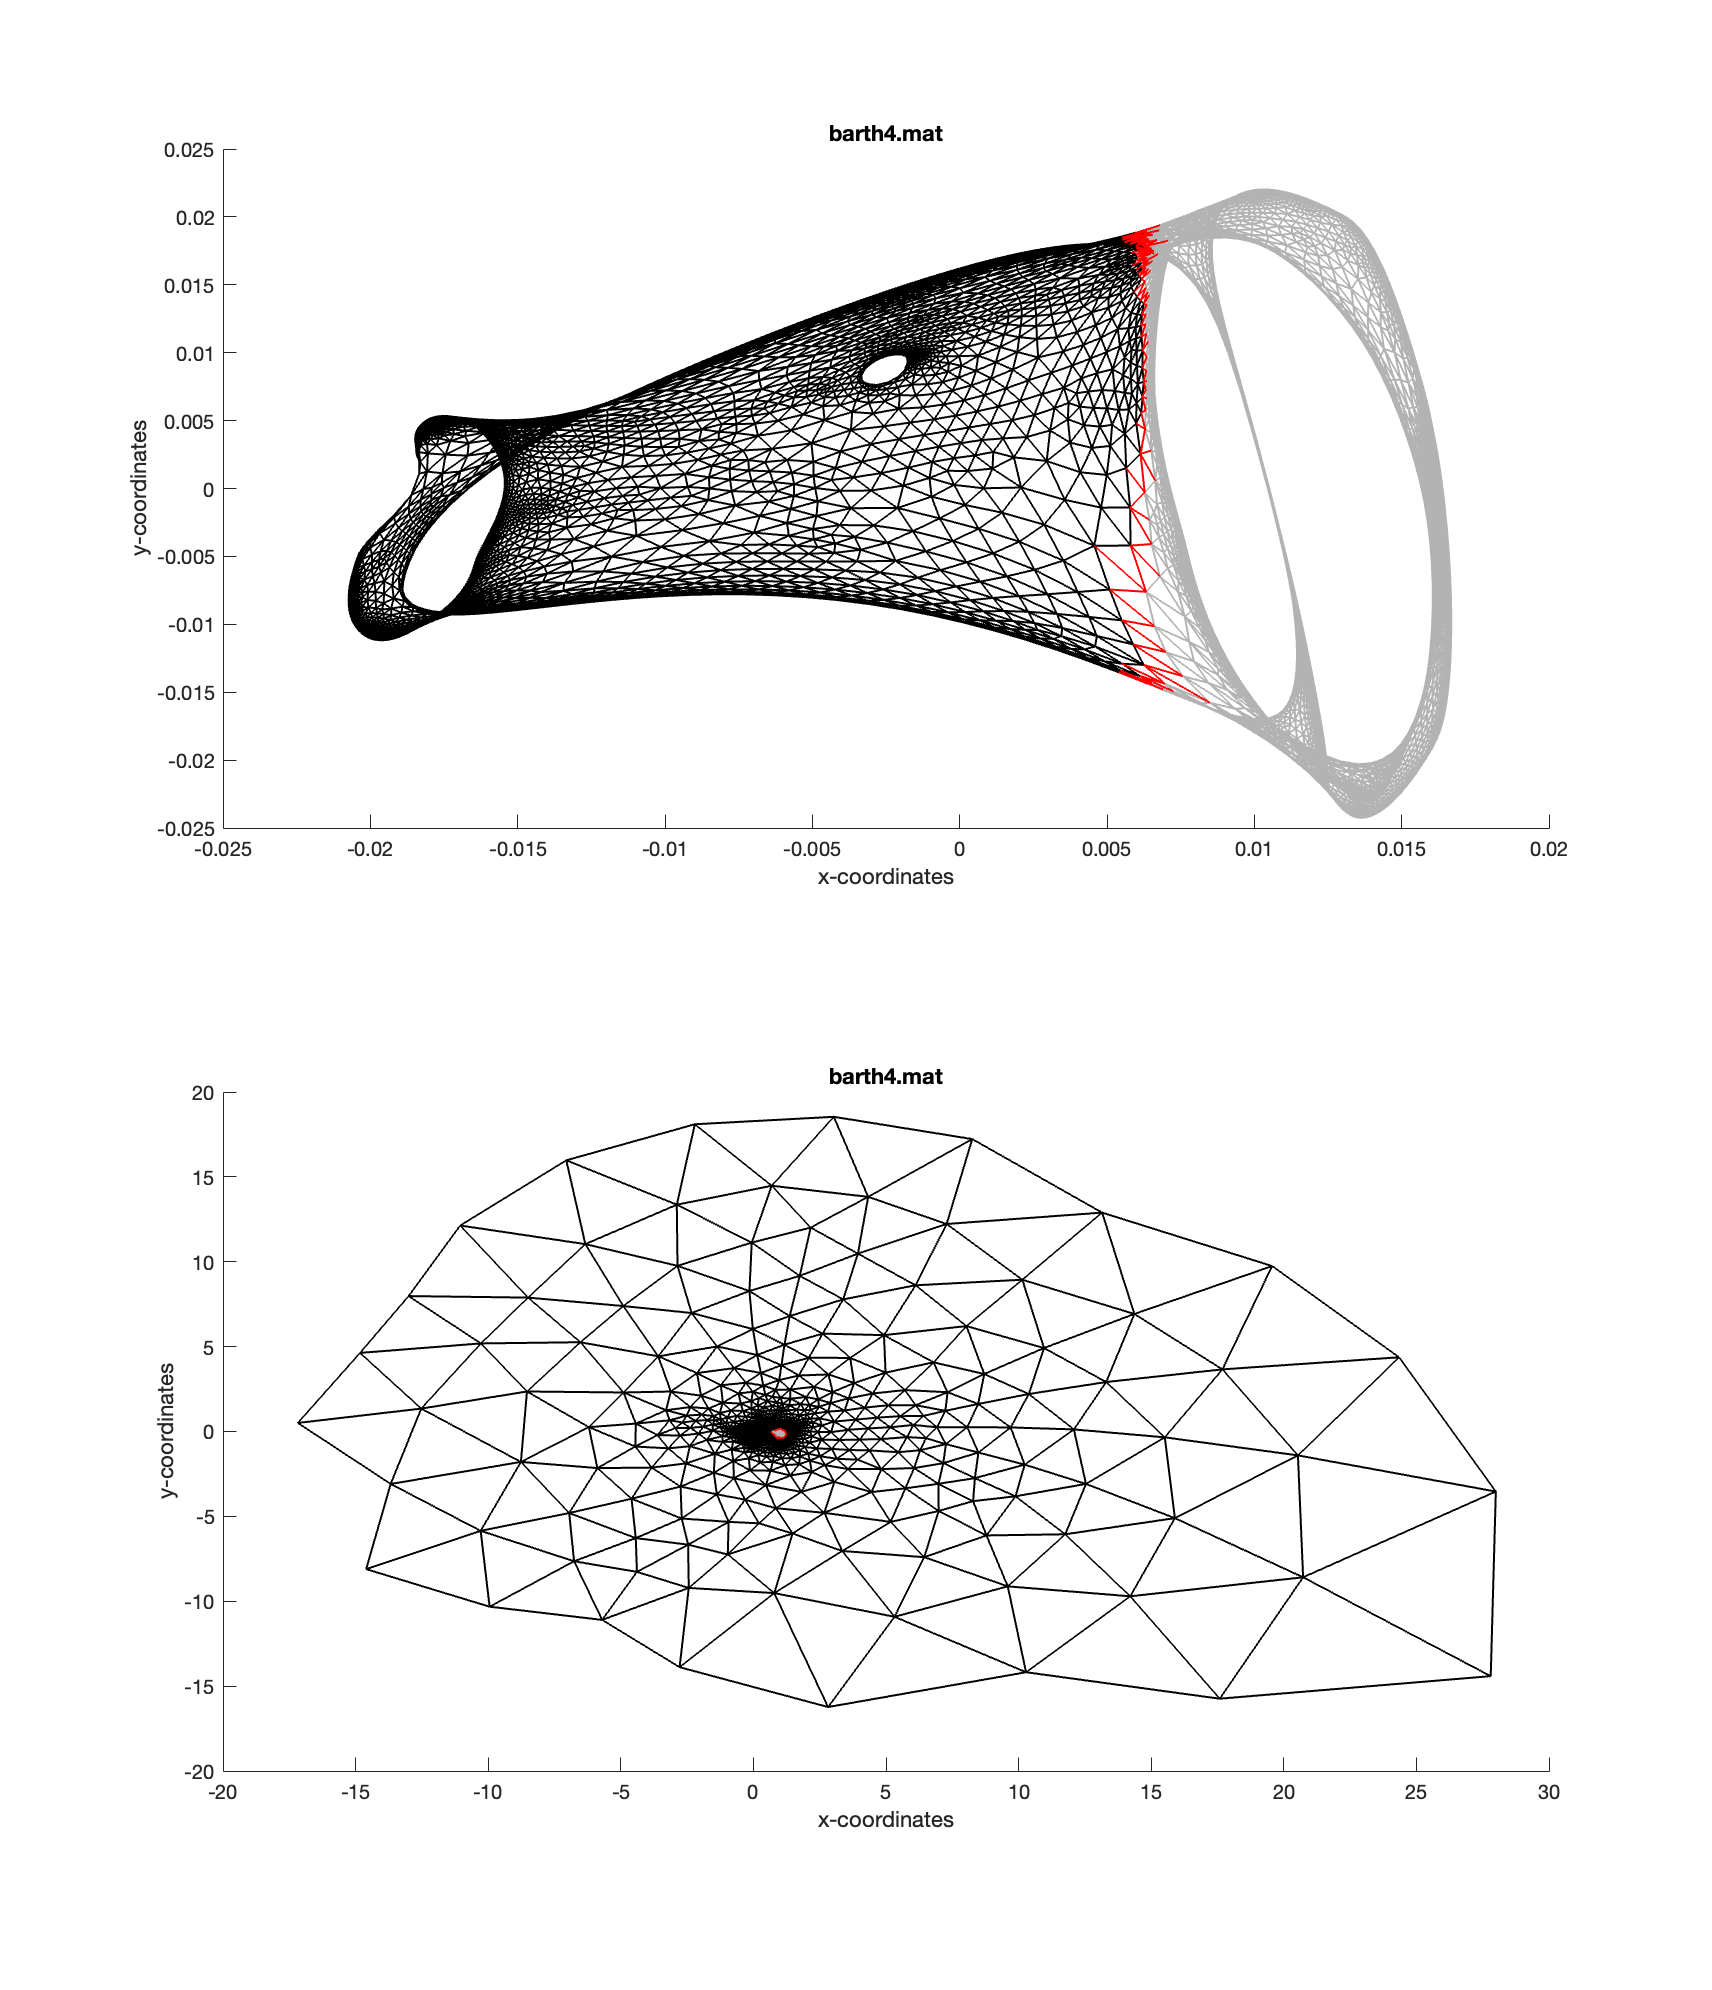
\includegraphics[width=\textwidth]{./media/barth4_eigen.png}
		\caption{barth4}
		\label{fig:coord_crack}
	\end{subfigure}\\
	\begin{subfigure}{0.5\textwidth}
		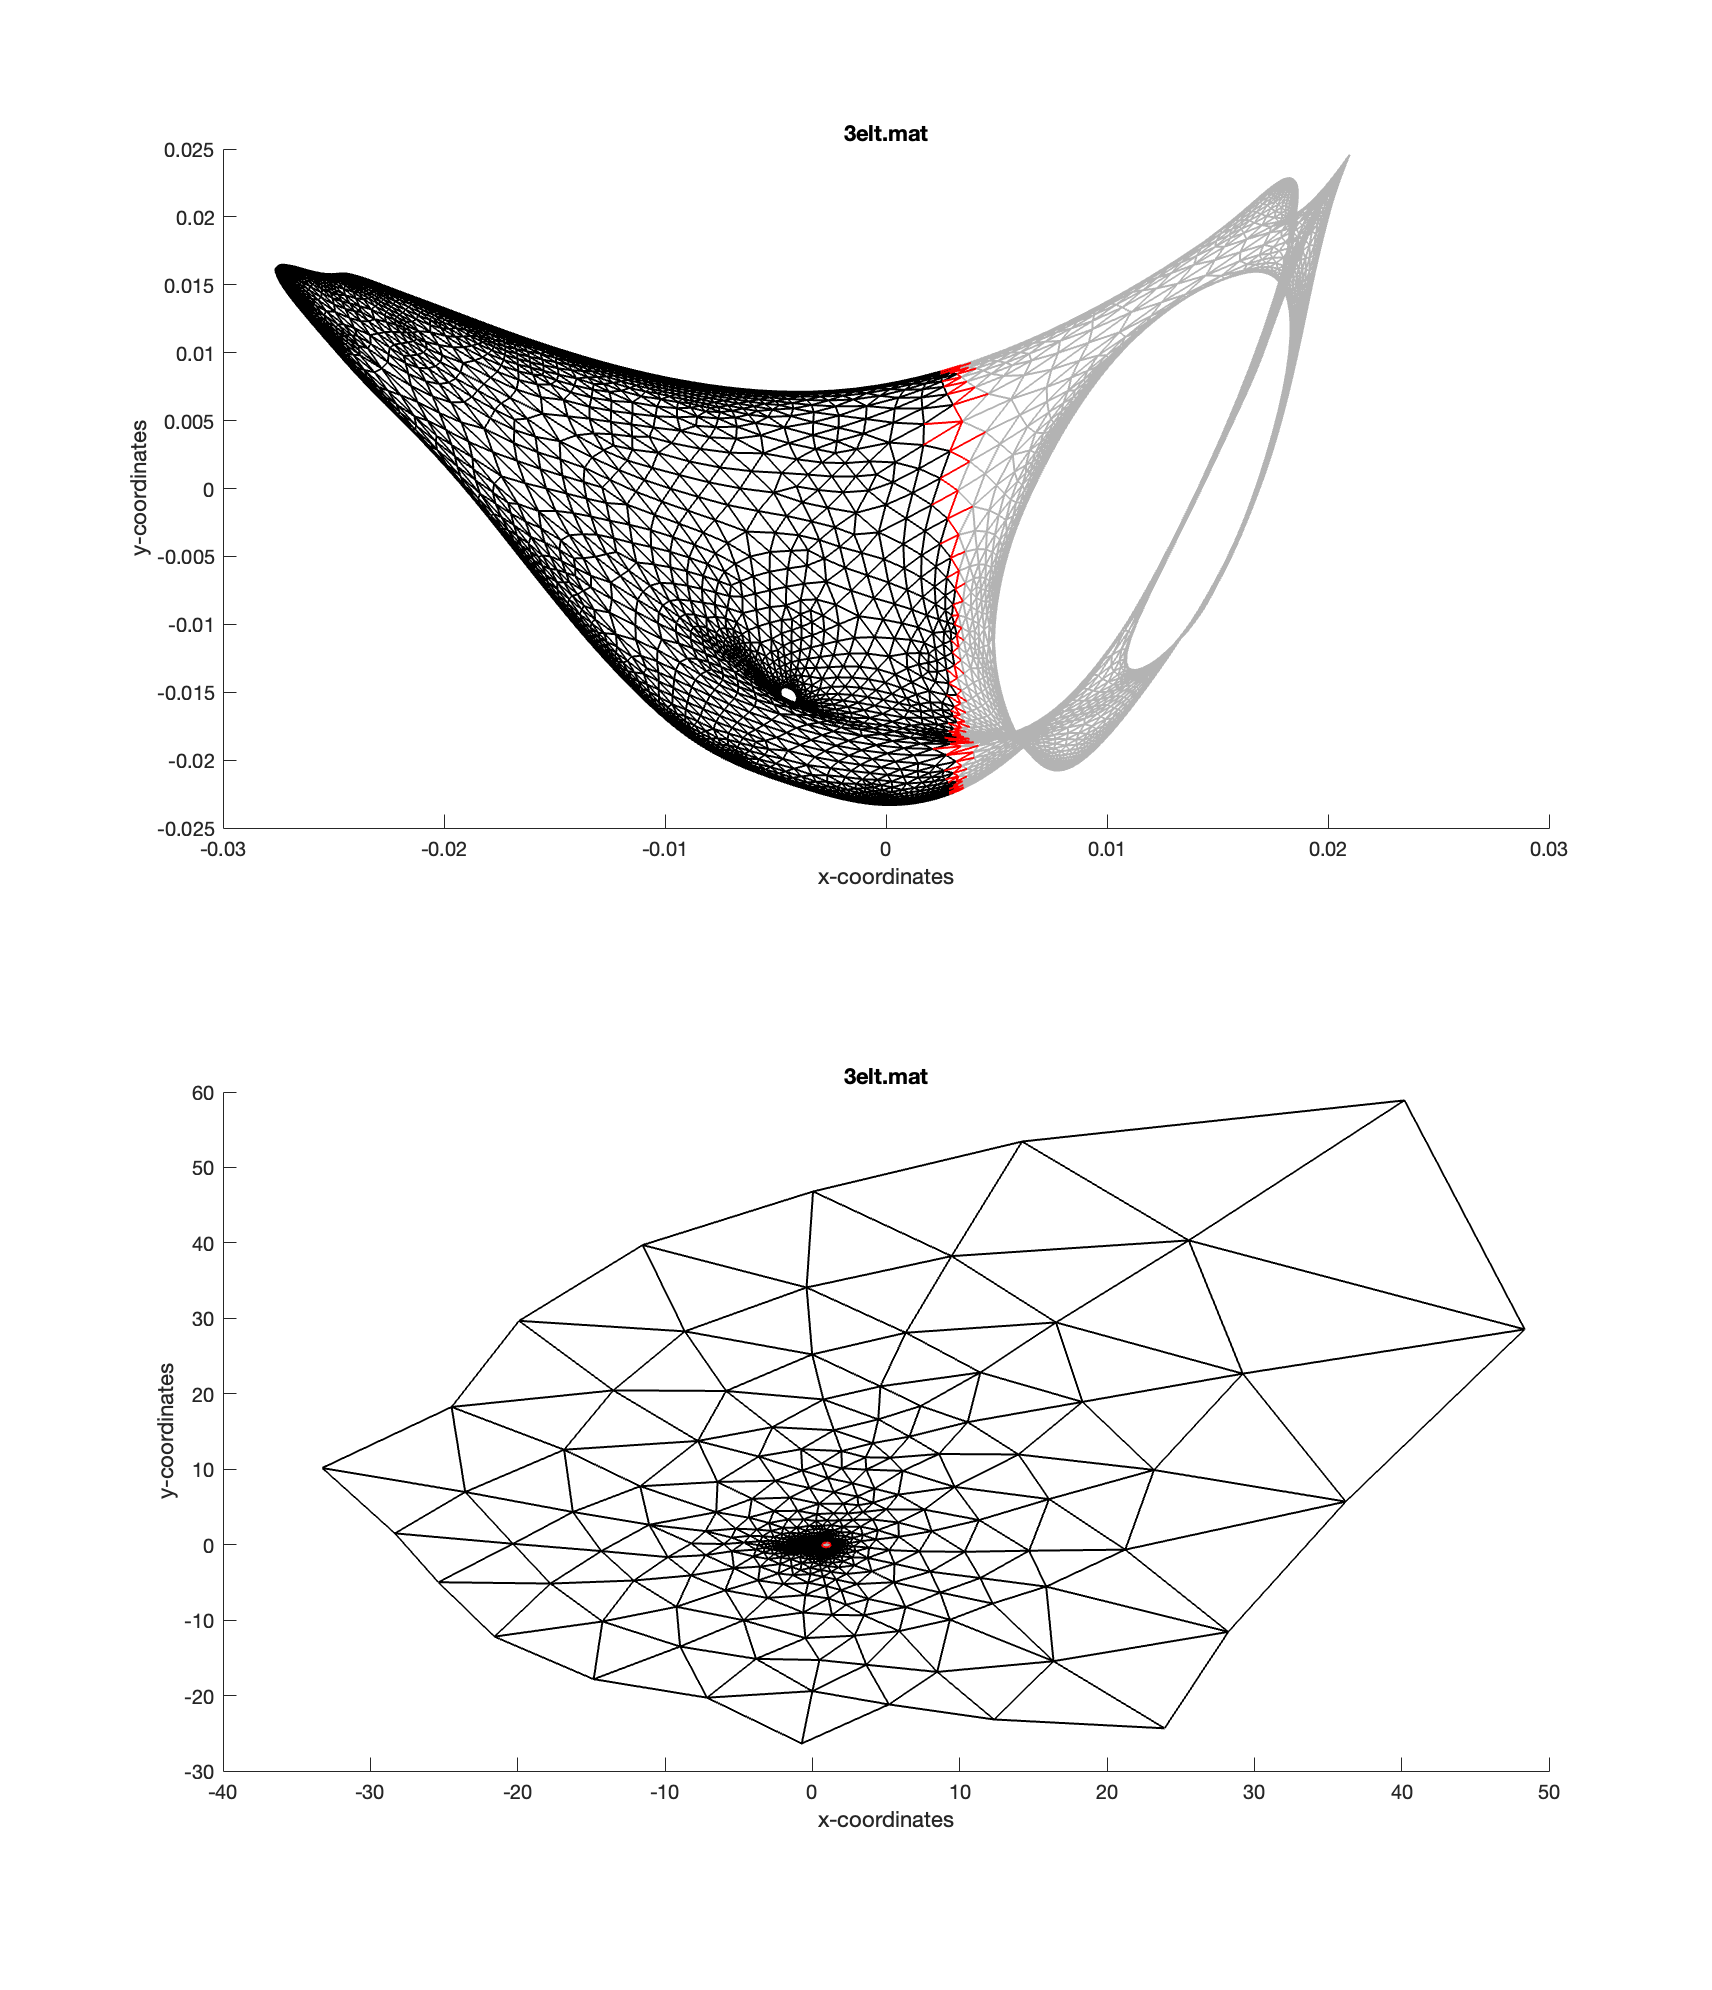
\includegraphics[width=\textwidth]{./media/3elt_eigen.png}
		\caption{3elt}
		\label{fig:metis_crack}
	\end{subfigure}%
	~
	\begin{subfigure}{0.5\textwidth}
		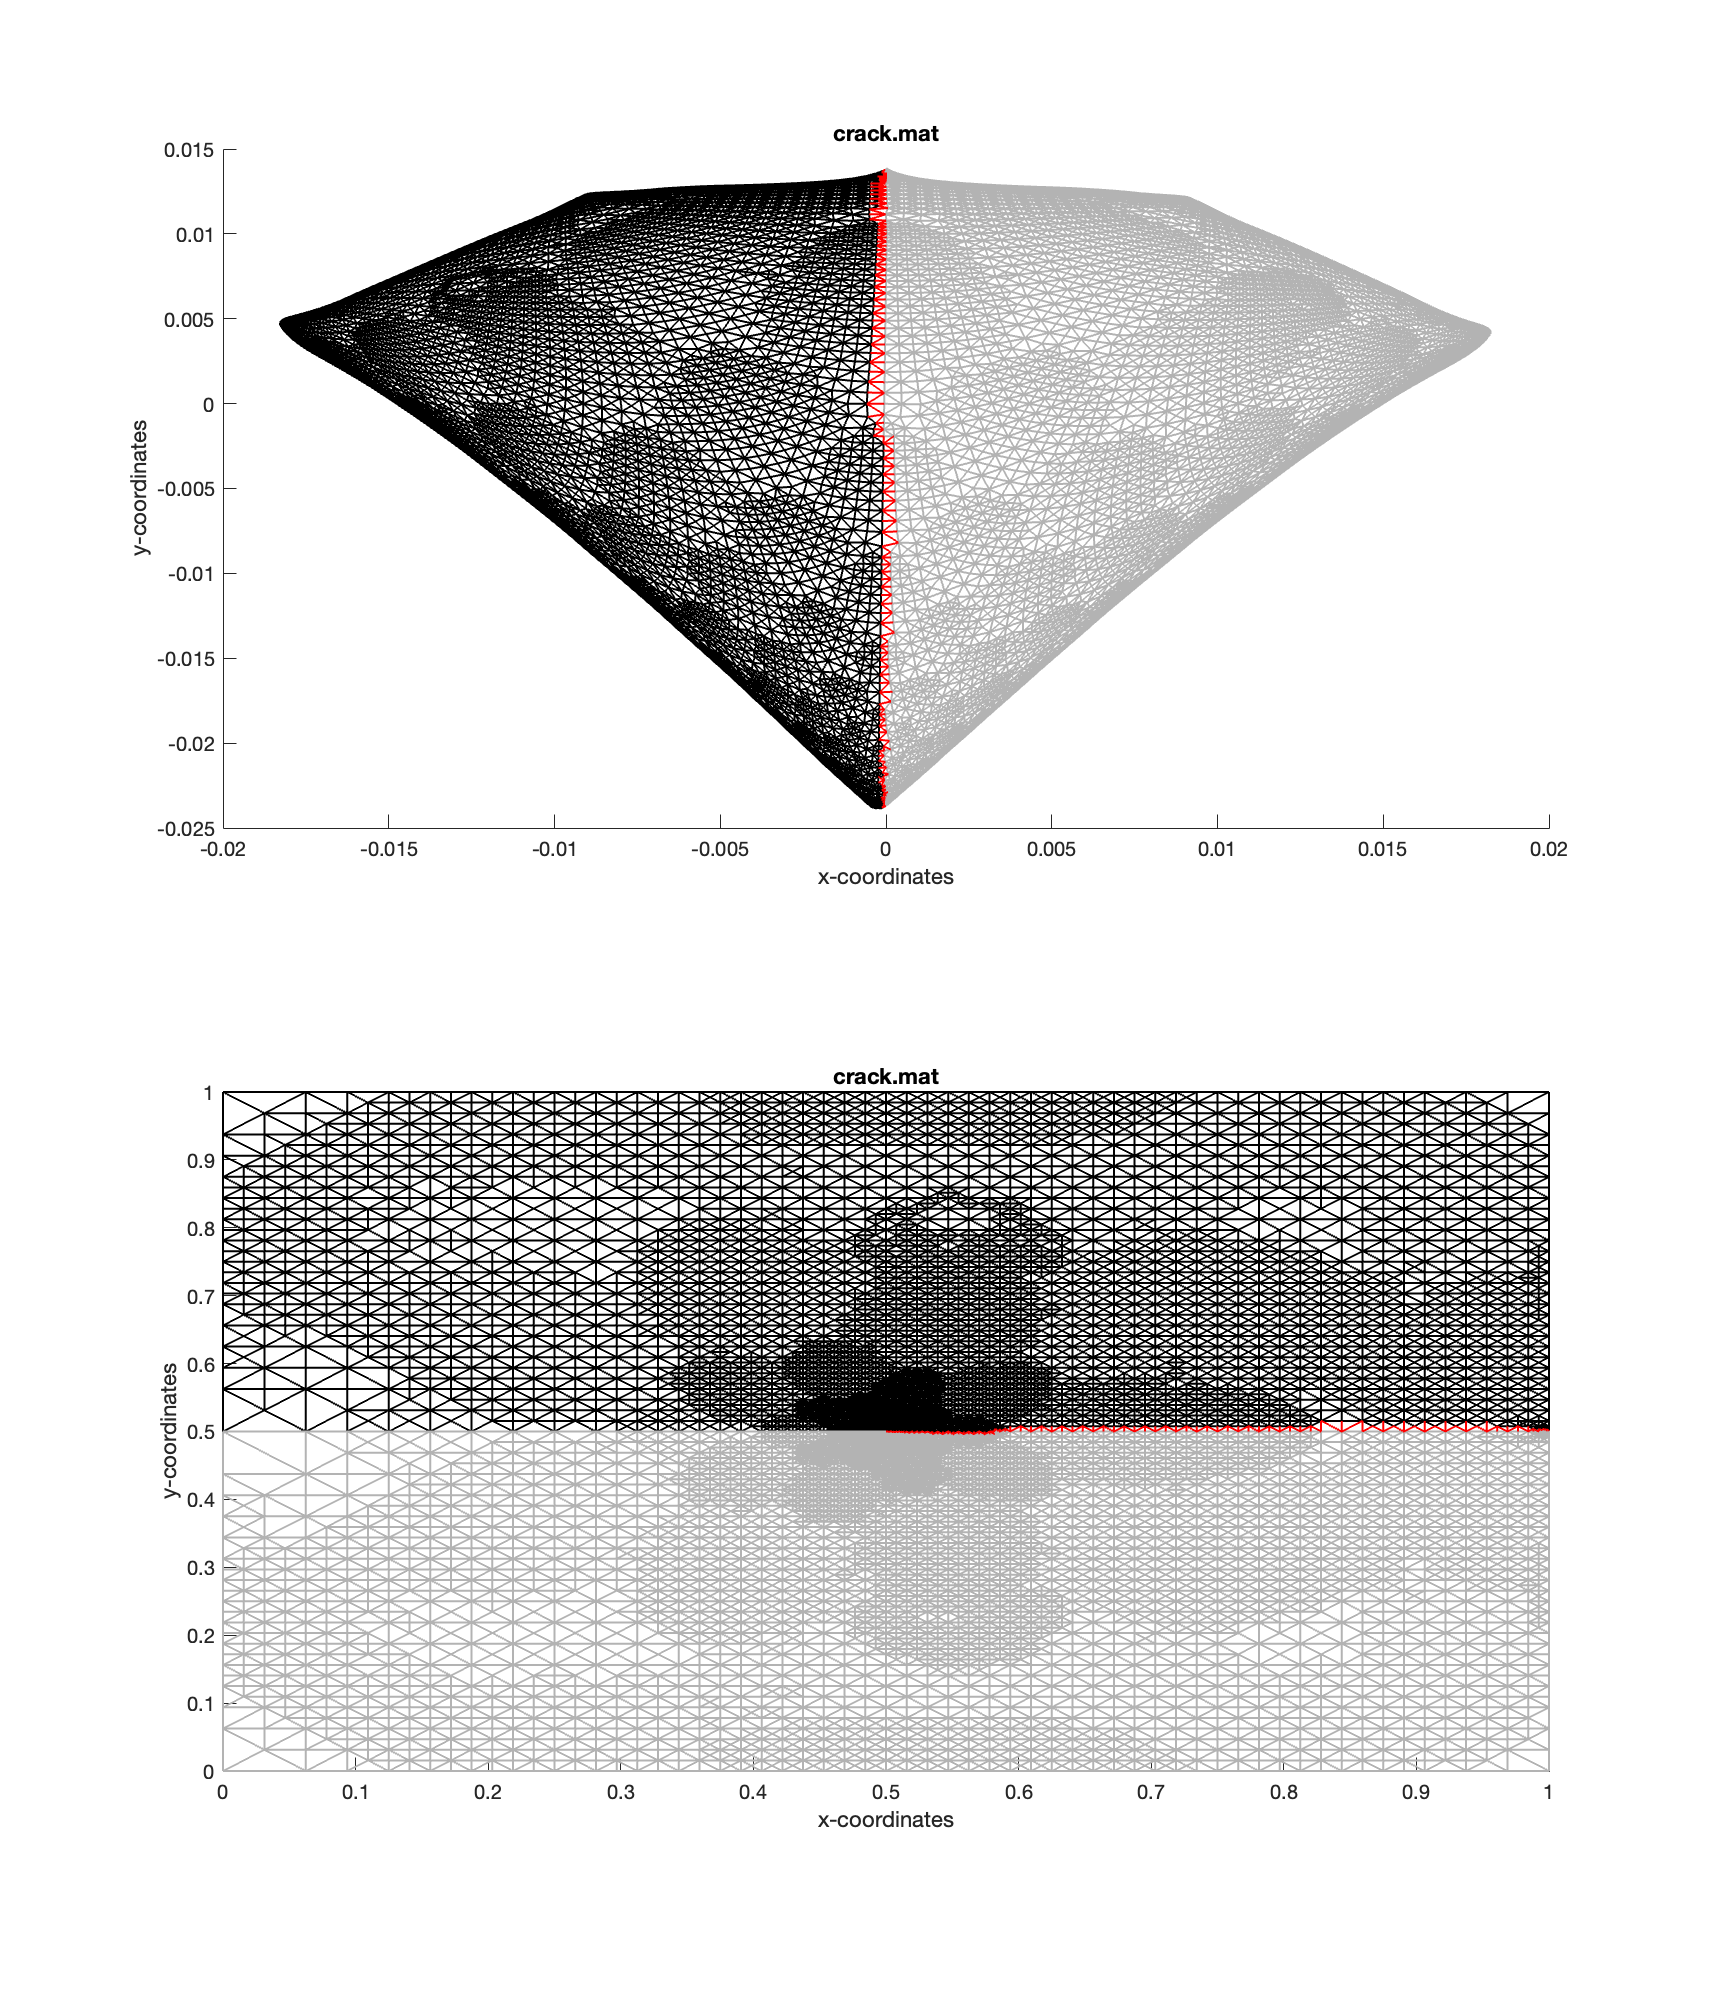
\includegraphics[width=\textwidth]{./media/crack_eigen.png}
		\caption{crack}
		\label{fig:inert_crack}
	\end{subfigure}
	\caption{Spectral bi-partitioning results using the eigenvectors to supply coordinates (top) and using cartesian coordinates (bottom).}
	\label{fig:rec_bi}
\end{figure}

